\documentclass[12pt,fleqn]{article}\usepackage{../../common}
\begin{document}
Ders 29

[onceki ders tekrari atlandi]

Uzaklaşım teorisinin ispatına gelelim. Bu ispatın daha kolay versiyonunu
yapacağım şimdi, tüm eşitlik yerine

$$
\int \oint_S < 0,0,R > \cdot \hat{n} \ud S =
\iiint_D R_z \ud V
$$

eşitliğinin ispatını yapacağım. Buradan hareketle daha genel eşitliği
ispatlamak kolay, aynı ispatı sadece $x$, sadece $y$ bileşeni olan
vektör alanları için tekrarlarım, ve tüm bunları toplayınca ana eşitliği
elde etmiş olurum.

İkinci bir basitleştirme yapalım, çünkü ispatı hala herhangi bir yüzey için
yapabileceğimden emin değilim. Dikey, basit bir yüzey kullanacağım, öyle ki
bu yüzey üzerinden entegralde $z$ değişkenin sınırlarını kolay halledebileyim.

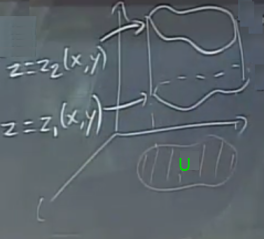
\includegraphics[width=15em]{calc_multi_29_01.png}








\end{document}
